\addPartText{Documentation du projet MySensors}
\part{Projet MySensors}

\chapter{Introduction}

\section{Présentation}

Ce document a pour but d'expliquer la mise en place d'une passerelle et d'une sonde MySensors.

\subsection{Organigramme}

\begin{figure}[h]
  \centering
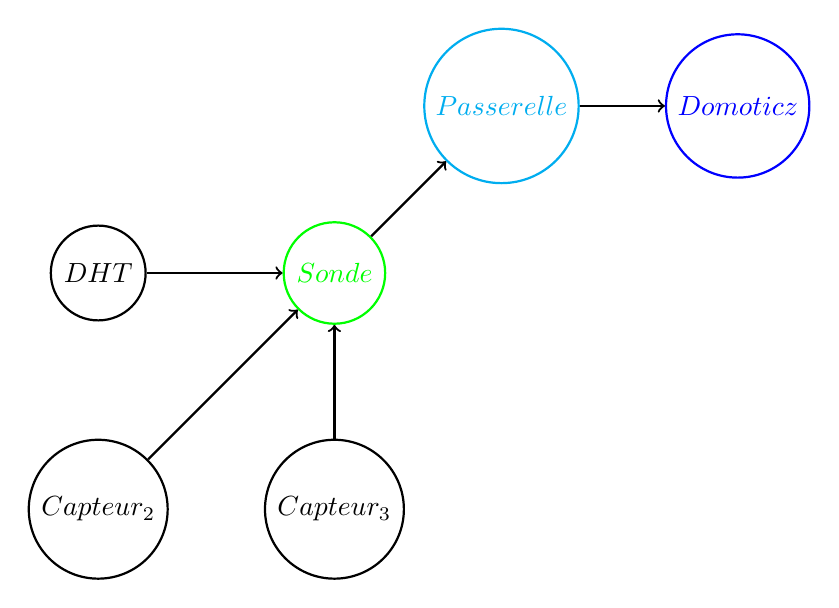
\begin{tikzpicture}[node distance={30mm}, thick, main/.style = {draw, circle}]
  \node[main] (1) [color=green] {$Sonde$}; 
  \node[main] (2) [above right of=1, color=cyan] {$Passerelle$}; 
  \node[main] (3) [left of=1] {$DHT$}; 
  \node[main] (4) [below of=3] {$Capteur_2$}; 
  \node[main] (5) [below of=1] {$Capteur_3$}; 
  \node[main] (6) [right of=2, color=blue] {$Domoticz$};
  
  \draw[->] (3) -- (1);
  \draw[->] (4) -- (1);
  \draw[->] (5) -- (1);

  \draw[->] (1) -- (2);
  \draw[->] (2) -- (6);
\end{tikzpicture} 
\caption{Les différents composants du projet}
\end{figure}

  \subsection{Principe}

  Les capteurs vont être analysés par la sonde MySensors.\\
  Cette dernière enverra à distance les informations vers la passerelle qui se chargera d'envoyer les informations au serveur Domoticz via une liaison USB.\\


  Une sonde représente un endroit physique, un lieu de mesure. \\
  Si vous souhaitez par la suite faire d'autres relevés dans un endroit différent, il suffira d'ajouter une sonde et de garder la passerelle.\\
  Chaque sonde est caractérisée par un identifiant de noeud (NODE\_ID) et chaque capteur possède un identifiant enfant sur la sonde qui lui est rattachée (CHILD\_ID)
  \begin{figure}[h]
    \centering
  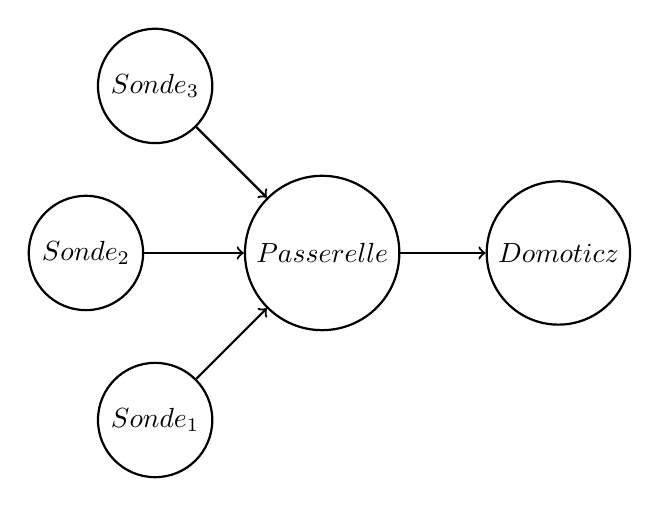
\begin{tikzpicture}[node distance={30mm}, thick, main/.style = {draw, circle}]
    \node[main] (1) {$Passerelle$}; 
    \node[main] (2) [below left of=1] {$Sonde_1$}; 
    \node[main] (3) [left of=1] {$Sonde_2$}; 
    \node[main] (4) [above left of=1] {$Sonde_3$}; 

    \node[main] (5) [right of=1] {$Domoticz$};
    
    \draw[->] (2) -- (1);
    \draw[->] (3) -- (1);
    \draw[->] (4) -- (1);
  
    \draw[->] (1) -- (5);
    \end{tikzpicture} 
    \caption{Une extension possible}
  \end{figure}





  \section{Structure du projet}

  Nous vous invitons à garder la structure suivante pour le projet : 
  
  Dans un dossier \lblue{DIR}{Domoticz\_Crepp}, placez deux dossiers appelés \lblue{DIR}{Sonde\_MySensors} et \lblue{DIR}{Passerelle\_MySensors}
  
  Ces deux derniers dossiers contiendront respectivement le programme de la sonde et de la passerelle.
  
  
  \begin{figure}[h!]
    \centering
  \usetikzlibrary{trees}
  
  \tikzstyle{every node}=[draw=black,thick,anchor=west]
  \tikzstyle{selected}=[draw=blue,fill=blue!30]
  \tikzstyle{optional}=[dashed,fill=gray!50]
  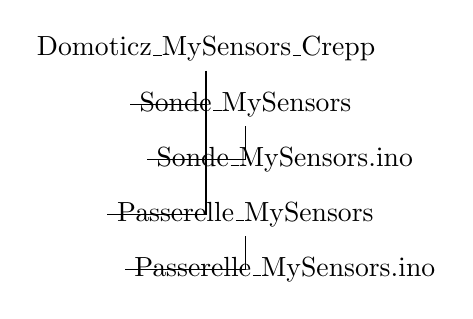
\begin{tikzpicture}[%
    grow via three points={one child at (0.5,-0.7) and
    two children at (0.5,-0.7) and (0.5,-1.4)},
    edge from parent path={(\tikzparentnode.south) |- (\tikzchildnode.west)}]
    \node {Domoticz\_MySensors\_Crepp}
      child { node {Sonde\_MySensors}
        child { node [selected] {Sonde\_MySensors.ino}}
      }
      child [missing] {}				
      child { node {Passerelle\_MySensors}
        child { node [selected] {Passerelle\_MySensors.ino}}
      };
  \end{tikzpicture}
  
  \tikzstyle{every node}=[]
  \tikzstyle{selected}=[]
  \tikzstyle{optional}=[]
  \caption{Arborescence du projet}
  \end{figure}

  Occupons nous maintenant des bilbiothèques Arduino.